\subsection{Lane Tracking}

To be able to calculate the distance between the POV and the lane, the lane has to be found in the video frame by frame. This could be done manually by the user or automatically by a software. The first option is easier to implement in a tool, but is a time-consuming task for the user. The second option is more demanding to implement, but if done correctly, could speed up the annotation process and provide more data to be used for analysing and model driver behaviour. The development process of the two lane detection methods, manual tracking and automatic tracking, are presented in this section.  

\subsubsection{Manual Tracking}

In this method, the lanes are defined manually by the user through marking points on the left and the right lanes in the video frames. The coordinates of these points were then used to calculate a linear line through the aforementioned points. To speed up this process, the user can define the lanes in one frame (possibly, the initial frame), skip through multiple frames, and define the lanes again (possibly, in the last frame). The program will then interpolate the lane placement and draw a an approximation of the lane placement on every frame between these two frames. The user will now be able to view all the frames with the drawn approximated lane and make changes in the markings of the points if the approximation of the lane position is not correct. 


\subsubsection{Automatic Tracking}
The aim was to develop a robust lane detection algorithm that required little manual work from the user. Robust in this case means that the lane detection should work well with both low and high quality NDS videos. Also, it should work well on videos recorded both during the day and during the night. All the steps involved in the development process of the lane detection algorithm are described below. An important remark is that  the algorithm is based on the one described in the literature review, section 1.3.2, but different approaches were tested in order to make the lane detection as good as possible. Three different definitions of region of interest was tested, this is presented later in this section. Also, Four different colour scales were tested, which are also presented later in this section. 

An overview of the developed automatic lane detection algorithm is presented in figure \ref{fig:my_label}. All steps in the development process of the algorithm are described below.

\begin{figure}[H]
    \centering
    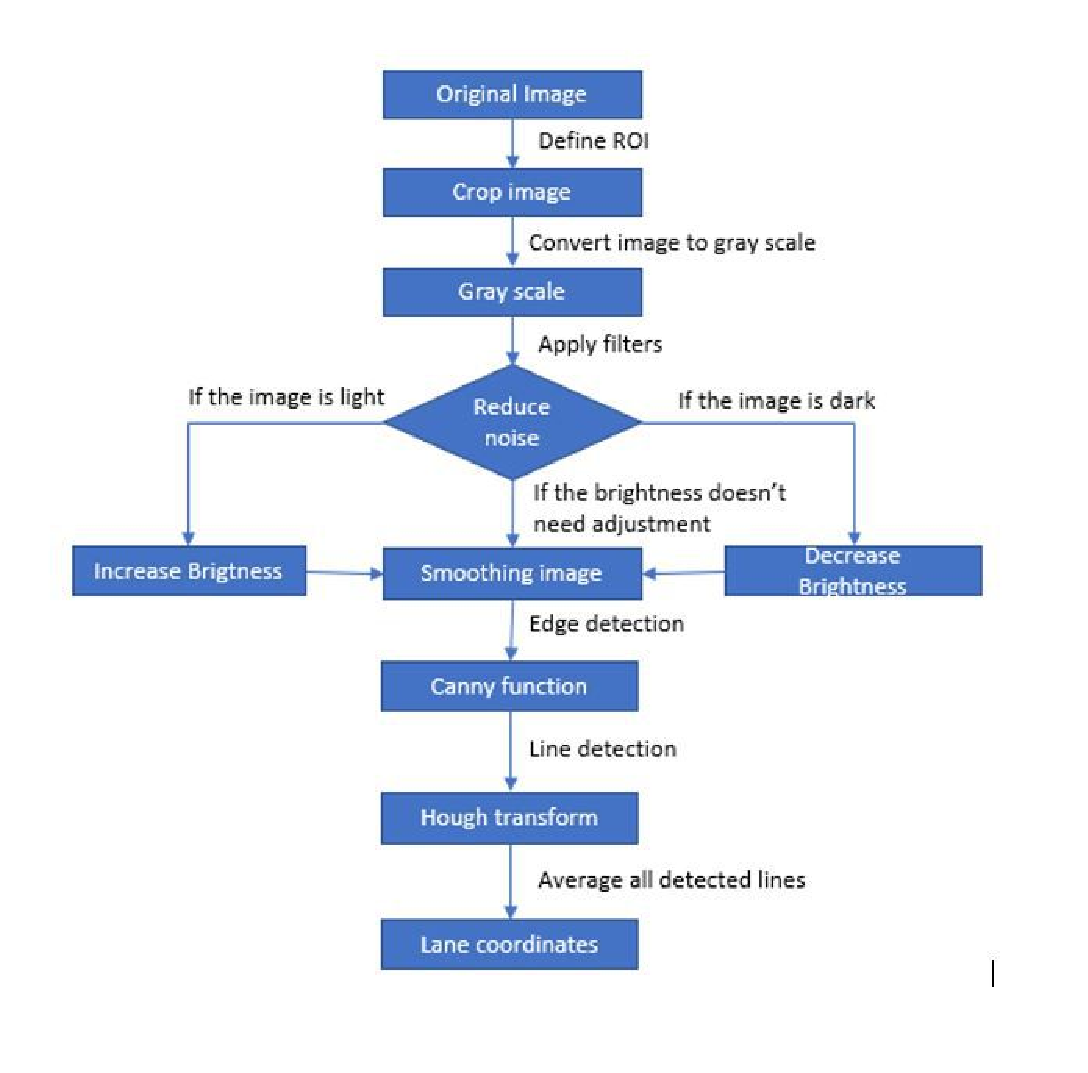
\includegraphics[width=\textwidth]{Figures/Algorithm.pdf}
    \caption{Final algorithm based on results obtained after masking}
    \label{fig:my_label}
\end{figure}

\paragraph{Region of Interest}

The first thing to do in order to detect the lanes in one frame is to define the Region Of Interest (ROI). The ROI contains all the interesting information in an image, in this case the area where the lanes are, and ensure that all the unnecessary information is ignored. A well-defined ROI contains as little unnecessary information (such as the landscape around the road, the road shoulders and other vehicles) as possible. Since the aim is to make the lane detection as automatic as possible, the ROI needs to be define with as little user input as possible. The different ROI:s that were considered for the algorithm are described below, together with their respective pros and cons.

\subsubsection*{ROI 1: Lower half of the image}
The ROI is defined as the bottom half of the image, like the region in red marking in Figure \ref{fig:my_ROI}. The positive aspect of this ROI is that the user doesn’t need to manually define the ROI. However, the ROI will contain a lot of unnecessary information, such as the landscape around the road, the road shoulders and the road between the lanes. This will lead to problems later when its time to detect the lanes. 

\subsubsection*{ROI 2: Triangular shape}
The ROI is defined as a triangle that contains the whole road, like the region in black marking in Figure \ref{fig:my_ROI}. This ROI needs to be defined by the user in the beginning of the annotation for the first frame, but the same ROI can be used in the upcoming frames. Assumed that the road doesn’t have any sharp turning during the event of interest, the same ROI can be used for the whole video.

\subsubsection*{ROI 3: Focus on one lane}
The ROI is defined as a small rectangle that mainly contains one of the lanes, like the region in blue marking in Figure \ref{fig:my_ROI}. This ROI needs to be defined by the user for at least two frames, the idea is that the user defines a ROI for the first frame and then define a new ROI for a frame a couple of time steps later. The ROI is then interpolated between the two frames and automatically updated for every frame. The number of frames for which the interpolation  can be applied depends on the shape of the road. If the road has a sharp turn, the user needs to define the ROI for more frames compared to a relative straight road. Also, the user needs to define one ROI for both the left and the right lane. This type of ROI consist of little unnecessary information, which will be helpful later when it is time to detect the lanes.

After trying all three types of ROI, the ROI focused on one lane successfully detected the most number of lanes and is therefore then one used in the lane detection algorithm.



\begin{figure}[H]
    \centering
    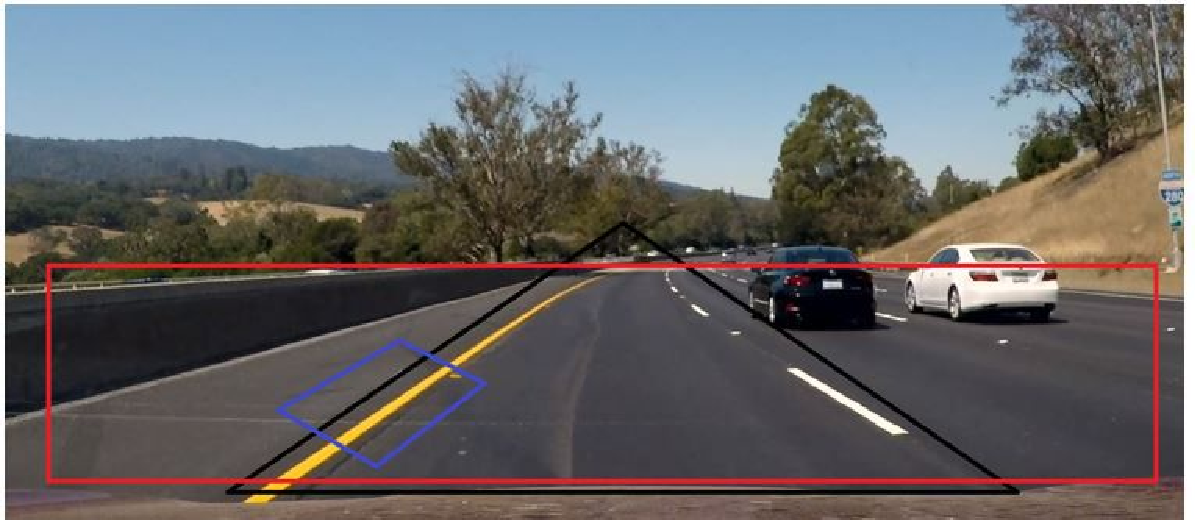
\includegraphics[width = 0.6\textwidth]{Figures/ROI_new.pdf}
    \caption{Approach to selecting different Region of interest}
    \label{fig:my_ROI}
\end{figure}

\paragraph{Colour selection}

The next step is to detect all the edges of lanes in the defined ROI for all the frames. As described in the literature review, section 1.3.2, the edges in an image is found by looking at the rapid change in intensity from two adjacent pixels. The intensity can be amplified and therefor make the edges more easy to detect by using different colour scales and mask out certain colours. In this case, the boundary of the yellow or white lanes and the gray asphalt is what defines the lanes and should be detected. The sections below describe different colour scales and how effective they are in amplifying the pixel intensity.

\subsubsection*{Color selection: Grayscale}
It is easy for the human eye to differentiate the gray asphalt from the yellow or white lanes, but due to shadows, complex lightning and worn out lanes (which change the pixels intensity on the road), it can be hard for a computer to distinct between the white/yellow lane and the road surface. Using a grayscale filter to convert the original RGB image to an image which consist of different shades of gray will reduce the shadows and lightning's influence and hence make the distinction between lanes and road surface clearer. Figure \ref{fig:color_scale} (top right) shows the original image after a grayscale filter been applied.

\subsubsection*{Color selection: Colour scales}
An alternative method to detect lanes is to filter out all the colours in the image except for the colours that the lane has, namely yellow and white. Different colour scales have different colour contrast, and a higher colour contrast makes it easier for a computer to detect a certain object with a certain colour. The different colour scales which was investigated during this work was RGB, HSV and HSL.  The original RGB image, which can be seen in figure \ref{fig:color_scale} (top left) was converted to a HSV image and HSL image, shown in figure \ref{fig:color_scale} (bottom right and bottom left respectively). The threshold values for yellow masking and white masking for the different colour scales are shown in table \ref{tab:Colour_conversion}. 

\begin{table}[H]
    \centering
    \begin{tabular}{c|c|c|c|c}
         \multicolumn{5}{c}{\textbf{Colour conversion}} \\ \hline
         Colour scale & Lower white & Upper white & Lower yellow & Upper yellow \\ \hline
         RGB & 160, 160, 160 & 255, 255, 255  & 150, 150, 0  & 255, 255, 80\\
         HSV & 0, 0, 160 & 0, 0, 255  & 60, 255, 150  & 60, 175, 255 \\
         HSL & 0, 0, 160 & 0, 0, 255  & 60, 255, 75  & 60, 255, 170
    \end{tabular}
    \caption{Threshold for yellow and white masking for different colour scales}
    \label{tab:Colour_conversion}
\end{table}


\begin{figure}[H]
    \centering
    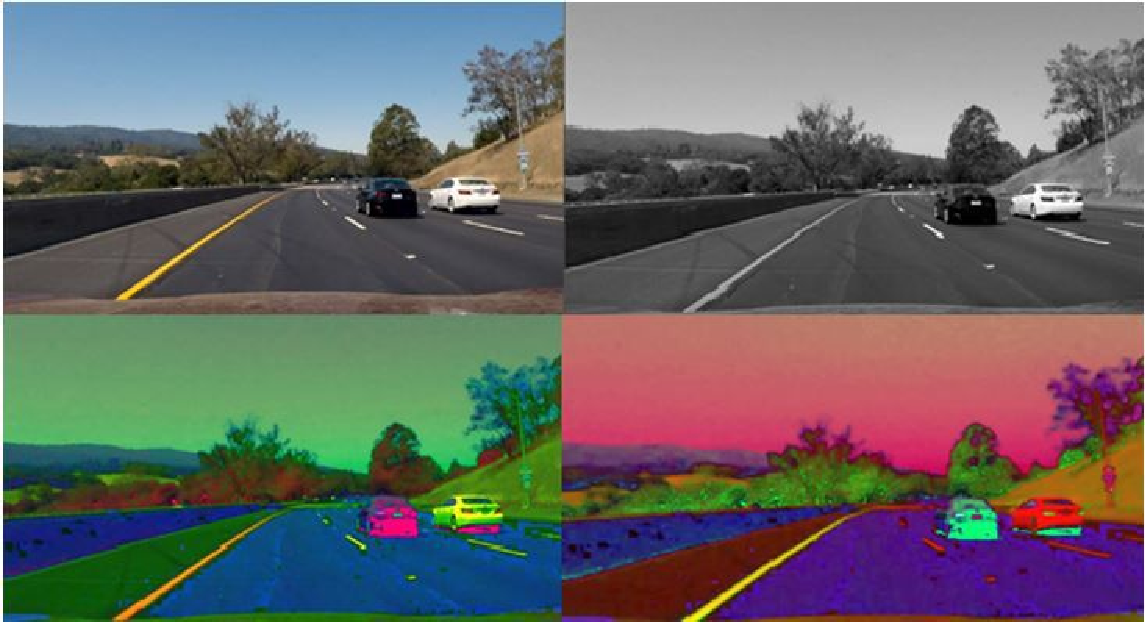
\includegraphics[width = 0.8\textwidth]{Figures/colorscale_2.pdf}
    \caption{Image conversion on different color scale}
    \label{fig:color_scale}
\end{figure}

\paragraph{Filters}
In order to obtain a correct detection of objects in an image, it is first necessary to distinguish them correctly. The noise and details in an image are reduced using a well known filter called Gaussian filter. The Gaussian filter is simple as it requires varying only one parameter; the variance. As seen in the equation below, it can be inferred that the amount of filtering is inversely proportional to the variance. Based on the level of suppression required on an image, the respective variance can be applied.
Other filters that can be considered are the mean-average and the median filters. Although they work well in reducing noise in an image faster than the Gaussian filter, they are ineffective in identifying the rate of change of frequency in an image which has sharp changes in colour.

\begin{equation} 
G(x,y)= \frac{1}{2\pi \sigma^2} e^ \frac{-x^2+y^2}{2\sigma^2}
\end{equation}
If the frame in which the lanes shall be detected is taken during night time, or if there are strong shadows in the frame, the brightness needs to be increased for better lane detection. And in the same way if the frame is taken during strong sunlight, the brightness needs to be decreased. The brightness and contrast of an image can be adjusted by applying a filter. In figure \ref{fig:lighter}, a filter is applied to the original dark frame, figure \ref{fig:lighter} (left), so the frame gets brighter, figure \ref{fig:lighter} (right), and therefor the lanes gets more visible. In figure \ref{fig:darker}, a filter is applied to the original light frame, figure \ref{fig:darker} (left), so the frame gets darker, figure \ref{fig:darker} (right), and therefor the lanes gets more visible.

\begin{figure}[H]
    \centering
    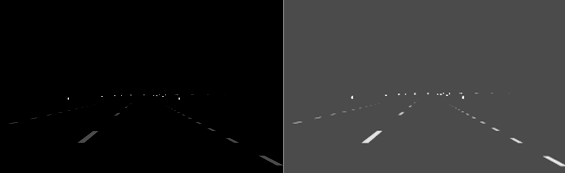
\includegraphics[width = 0.8\textwidth]{Figures/lighter.png}
    \caption{Increase the brightness of an image with a filter}
    \label{fig:lighter}
\end{figure}


\begin{figure}[H]
    \centering
    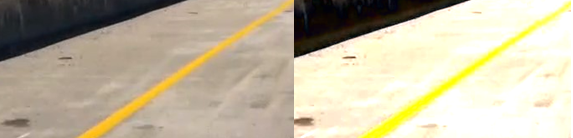
\includegraphics[width = 0.8\textwidth]{Figures/darker.png}
    \caption{Decrease the brightness of an image with a filter}
    \label{fig:darker}
\end{figure}


\paragraph{Canny edge detection}

The edges in the defined ROI are now ready to be detected. The edge detection is done with a canny function. The canny function was applied to all three different colour scales frames and the gray scale frame presented in figure \ref{fig:color_scale} and the result is presented in figure \ref{fig:canny}. The canny function applied to the original RGB image can be seen in figure \ref{fig:canny} (top left). The canny function applied to the converted HSV image and the converted HSL image can be seen in figure \ref{fig:canny} (bottom right and bottom left respectively). Finally, the canny function applied to the gray scale image can be seen in figure \ref{fig:canny} (top right).


\begin{figure}[H]
    \centering
    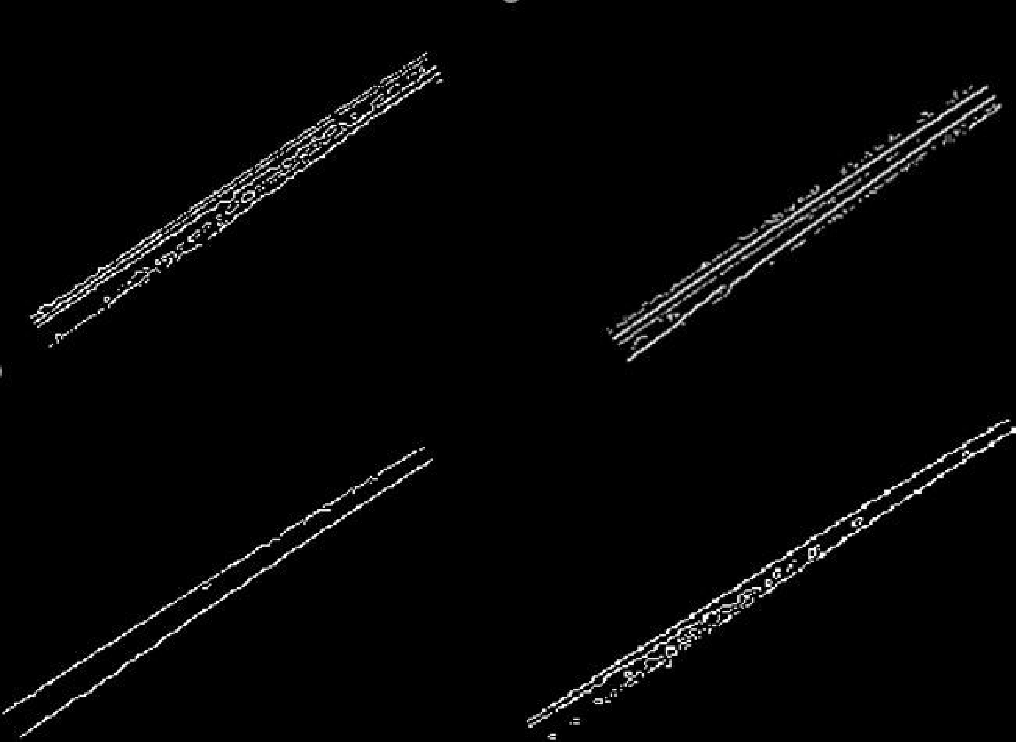
\includegraphics[width = 0.8\textwidth]{Figures/edge.pdf}
    \caption{Edge detection using canny operator}
    \label{fig:canny}
\end{figure}

\paragraph{Hough Transform}
\label{par:Hough_t}
Hough transform is a widely used  technique in computer vision and image analysis for feature extraction. Originally, it was used to identify lines but later was developed for other shapes as well. 
\begin{figure}[H]
    \centering
    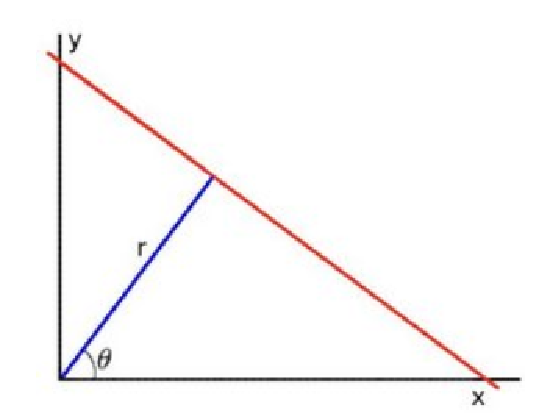
\includegraphics[width = 0.4\textwidth]{Figures/line_pol.pdf}
    \caption{A line in polar co-ordinates}
    \label{fig:Hough}
\end{figure}
Considering the equation of a line in polar co-ordinate system from Figure \ref{fig:Hough}, where $r$ represents the perpendicular distance to the line, ($\theta$) is the angle in radians with the X-axis and (x,y) are points on line for which $r$ and $\theta$ are constants.
\begin{equation}
    r = x cos(\theta) + y sin(\theta)
    \label{eq:Hough_eq}
\end{equation}
Since the variables (r,$\theta$) of the equation of line have to lie between definite values, the equation of line in Cartesian form can not be used as slope may take values up to infinity.
From the equation \ref{eq:Hough_eq},it can be inferred that for known points (x,y), the subsequent (r,$\theta$) can be plotted. Each point gives a sinusoidal curve in the (r,$\theta$) plane.The points which are collinear yield curves which intersect at common point (r,$\theta$)  This essentially forms the principle behind the Hough transform. The threshold can be set for the number of lines which intersect ar r and $\theta$. The Hough transform declares a line based on the set threshold. 



\paragraph{Averaging lines}
As seen in section \ref{par:Hough_t}, the Hough transform is used to identify which of the detected edges are part of a lane and reject those edges that are not part of a lane.  In the ideal case, the Hough transform identify two edges as parts of a lane, the vertical left and right side of the actual lane. The detected lanes position is estimated by taking the average slope and the average position in x,y- coordinates of the detected edges. In some cases however, the Hough transform misdetect an edge as part of a lane, which will lead to a worse estimation of the lanes position. In order to avoid misdetection of lanes, the algorithm only consider the edges which have a similar slope, that is maximum 60 degrees different, to the region of interest.  

The estimated lanes are drawn on the frame which are analysed so the user can visually determine if the estimation is accurate. Also, the estimated lanes end-points in x,y-coordinates are given as an output from the algorithm




\paragraph{Bird's eye perspective}
The image obtained from forward facing camera appears to converge to an infinite point in the image plane due to perspective. It is vital to correct this as it affects the parameters to be calculated. To change the perspective as viewed from the top gives a better understanding of the lanes, especially the curved ones.

The most commonly used technique is bird's eye transformation. This allows the image to be transformed such that it appears as seen from the top. This method could be an alternative to solving the heading angle problem. However, it's limitation is that only lanes are seen clearly where as objects are stretched in the vertical direction and may not useful in annotating cars. 


\subsubsection{Semi Automatic Tracking}
This method will let the user define the Region Of Interest in a couple of frames, then the lane detection algorithm described above could search for the lanes within this RIO. This would allow for faster annotation compared to manual annotation and better lane detection. 

\subsubsection{Test of Lane detection algorithm}

Some tests was performed in order to determine which of the colour scales gives the best result in terms of detecting lanes and should therefor be used in the final lane detection algorithm described in section 2.2.2. The four different colour scales, namely RGB, HSV, HSL and gray scale was tested on three different scenarios, NDS videos containing dashed lanes, NDS videos containing solid lanes and NDS videos recorded during night time. Three representative videos were used for each of the three scenarios and the results are presented in section 3.2. 

In order to check how trustworthy the lane detection algorithm is in the sense that the detected lanes are actually lanes and not something else, a misdetection test was performed. In the test, the ROI of the lane detection algorithm was defined in an area of the frame where no lanes are present, and the percentage of misdetected lanes was noted. The test was done both for videos recorded both during day time and videos recorded during night time. The results of this test are presented in section 3.2.

In order to check how accurate the lane detection are, a flickering test was performed. Flickering is the relative horizontal movement in pixels of the detected lane from one frame to the next frame. Lanes are used as an measuring rod for the vehicles position on the road, and high flickering creates the false impression the the vehicle has a lateral movement. The flickering test was performed for one NDS video recorded during day time and one NDS video recorded during day time and the result is presented in section 3.2.


